En cuestiones de medición del rendimiento, existe un repositorio de \textit{GitHub} muy popular utilizado por la mayoría de la gente que busca medir el rendimiento de su modelo de inteligencia artificial. Este repositorio es \url{https://github.com/rafaelpadilla/Object-Detection-Metrics.git}, posee un fichero \textbf{README.md} de vital importancia, en el que se explica todas las métricas que podemos obtener, su explicación teórica y cómo obtenerlas. Asimismo, proporciona dos ejemplos guiados para poder realizar pruebas sencillas. En nuestro proyecto se encuentra dentro de la tercera carpeta \textit{3_Rendimiento}.\\

Sin embargo, nosotros hemos realizado nuestro propio script \textbf{precisionVSrecall.py} para poder obtener la curva de Precisión vs Recuperación (\textit{Precision vs Recall}) que se encuentra dentro del directorio rendimiento. Mediante esta curva podremos evaluar el modelo. La precisión se refiere a la proporción de verdaderos positivos (TP) y falsos positivos (FP). La recuperación se refiere a la proporción de verdaderos positivos entre la suma de verdaderos positivos con falsos negativos. En definitiva, sirve para evaluar la calidad de un modelo de clasificación y se puede utilizar para determinar el umbral óptimo para el modelo.\\

La idea principal para obtener dicha curva es comparar la clase y cuadros de delimitadores de numerosas fotos etiquetadas y procesadas por el algoritmo de detección. Es decir, para una imagen comparar la señal real con la detectada. Se deben introducir todos los ficheros TXT con los datos de etiquetado en el interior de \textbf{rendimiento/images/groundtruths/} y los ficheros TXT con los datos de detección en el directorio \textbf{rendimiento/images/detections/}. Ejecutando entonces el script \textbf{precisionVSrecall.py} podremos obtener la curva de rendimiento:
\begin{lstlisting}
python3 precisionVSrecall.py
\end{lstlisting}

A modo de ejemplo, nosotros probamos con 64 imágenes y estos fueron los resultados que obtuvimos:

\begin{figure}[H]
	\centering
	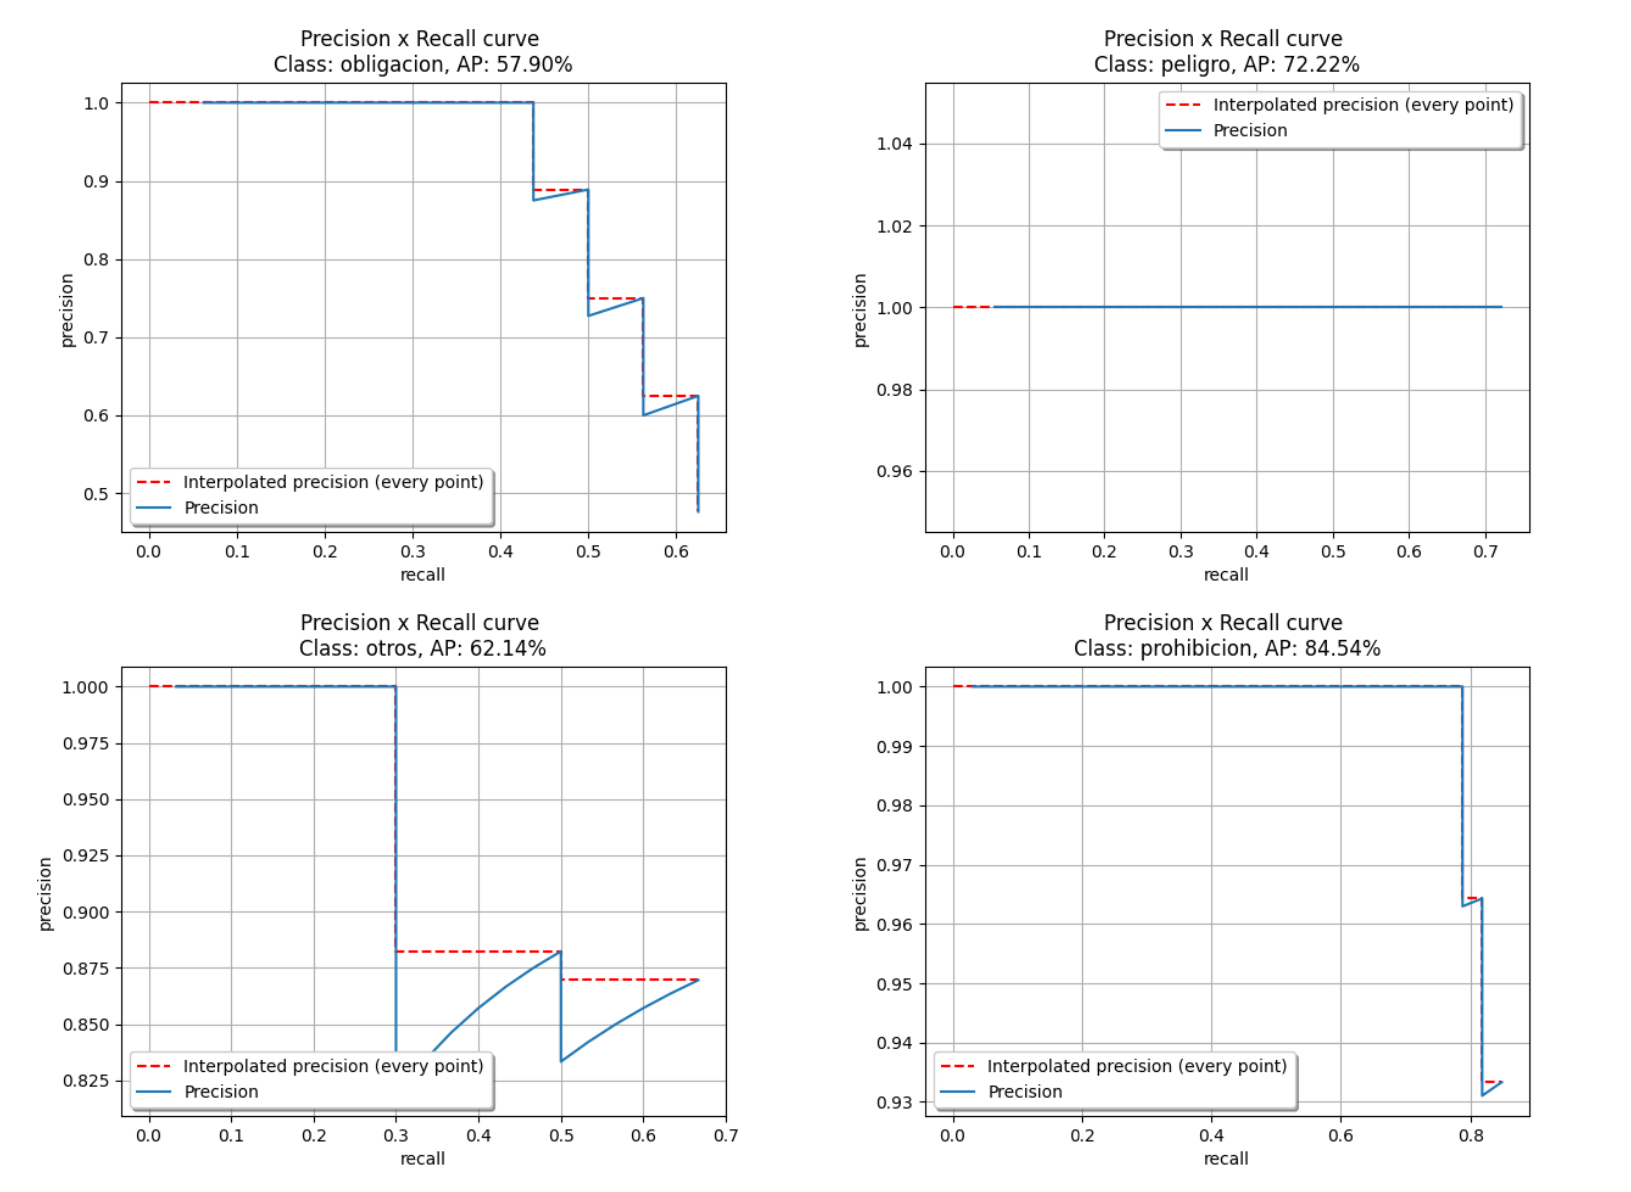
\includegraphics[width=\textwidth]{Imagenes/AnexoI_Manual/AA/rendimiento.pdf}
	\caption{Medida de rendimiento}
	\label{rendimiento}
\end{figure}


